%%%%%%%%%%%%%%%%%%%%%%%%%%%%%%%%%%%%%%%%%
% Beamer Presentation
% LaTeX Template
% Version 1.0 (10/11/12) 
%
% This template has been downloaded from:
% http://www.LaTeXTemplates.com
%
% License:
% CC BY-NC-SA 3.0 (http://creativecommons.org/licenses/by-nc-sa/3.0/)
%
%%%%%%%%%%%%%%%%%%%%%%%%%%%%%%%%%%%%%%%%%

%----------------------------------------------------------------------------------------
%	PACKAGES AND THEMES
%----------------------------------------------------------------------------------------

\documentclass{beamer}

\mode<presentation> {
%\mode<handouts> {
%\mode<article> {


% The Beamer class comes with a number of default slide themes
% which change the colors and layouts of slides. Below this is a list
% of all the themes, uncomment each in turn to see what they look like.


%\usetheme{default}
%\usetheme{AnnArbor}
%\usetheme{Antibes}
%\usetheme{Bergen}
%\usetheme{Berkeley}
%\usetheme{Berlin}
%\usetheme{Boadilla}
\usetheme{CambridgeUS}
%\usetheme{Copenhagen}
%\usetheme{Darmstadt}
%\usetheme{Dresden}
%\usetheme{Frankfurt}
%\usetheme{Goettingen}
%\usetheme{Hannover}
%\usetheme{Ilmenau}
%\usetheme{JuanLesPins}
%\usetheme{Luebeck}
%\usetheme{Madrid}
%\usetheme{Malmoe}
%\usetheme{Marburg}
%\usetheme{Montpellier}
%\usetheme{PaloAlto}
%\usetheme{Pittsburgh}
%\usetheme{Rochester}
%\usetheme{Singapore}
%\usetheme{Szeged}
%\usetheme{Warsaw}

% As well as themes, the Beamer class has a number of color themes
% for any slide theme. Uncomment each of these in turn to see how it
% changes the colors of your current slide theme.

%\usecolortheme{albatross}
\usecolortheme{beaver}
%\usecolortheme{beetle}
%\usecolortheme{crane}
%\usecolortheme{dolphin}
%\usecolortheme{dove}
%\usecolortheme{fly}
%\usecolortheme{lily}
%\usecolortheme{orchid}
%\usecolortheme{rose}
%\usecolortheme{seagull}
%\usecolortheme{seahorse}
%\usecolortheme{whale}
%\usecolortheme{wolverine}

%\setbeamertemplate{footline} % To remove the footer line in all slides uncomment this line
%\setbeamertemplate{footline}[page number] % To replace the footer line in all slides with a simple slide count uncomment this line

%\setbeamertemplate{navigation symbols}{} % To remove the navigation symbols from the bottom of all slides uncomment this line
}

\usepackage{graphicx} % Allows including images
\graphicspath{{../figures}}
\usepackage{booktabs} % Allows the use of \toprule, \midrule and \bottomrule in tables
\usepackage{amsmath, amssymb, amsthm, gensymb,mathrsfs}%,eufrak}
\usepackage{hyperref}
\usepackage{tabularx}
\usepackage{longtable}
\usepackage{makecell}
\usepackage{multicol}
\usepackage{physics}

\newcommand{\uvec}[1]{\textbf{#1}}

\newcounter{excounter}
%\renewcommand{\thefpcounter}{\thechapter.\arabic{fpcounter}}
%\renewcommand{\thefpcounter}{\thesection.\arabic{fpcounter}}
\renewcommand{\theexcounter}{\arabic{excounter}}

\newtheorem{teorema}{Teorema}[section]
\newtheorem{definicio}{Definició}[section]

\usepackage[lastexercise]{exercise}

\graphicspath{{../figures}}

%----------------------------------------------------------------------------------------
%	 TITLE PAGE
%----------------------------------------------------------------------------------------

\title[Regression]{Regression} % The short title appears at the bottom of every slide, the full title is only on the title page

\author{Jordi Villà i Freixa} % Your name
\institute[FCTE] % Your institution as it will appear on the bottom of every slide, may be shorthand to save space
{
Universitat de Vic - Universitat Central de Catalunya \\
Study Abroad\\ % Your institution for the title page
\medskip
\textit{jordi.villa@uvic.cat} % Your email address
}
%\date{\today} % Date, can be changed to a custom date
\date{course 2023-2024}
\logo{
\includegraphics[width=.1\textwidth]{FCTE}}
\begin{document}

\begin{frame}
\titlepage % Print the title page as the first slide
\end{frame}

\begin{frame}
\frametitle{Índex} % Table of contents slide, comment this block out to remove it
\tableofcontents % Throughout your presentation, if you choose to use \section{} and \subsection{} commands, these will automatically be printed on this slide as an overview of your presentation
\end{frame}

%----------------------------------------------------------------------------------------
%	PRESENTATION SLIDES
%----------------------------------------------------------------------------------------
\section{Introduction and scope}
\begin{frame}
  \frametitle{Preliminary note}
  The material in these slides is strongly based on \cite{kroese2020}. When other materials are used, they are cited accordingly.

  Mathematical notation follows as good as it can a \href{https://ctan.math.utah.edu/ctan/tex-archive/macros/latex/contrib/mlmath/mlmath.pdf}{good practices proposal} from the Beijing Academy of Artificial Intelligence.
  \end{frame}

%------------------------------------------------
\section{Introduction} % Sections can be created in order to organize your presentation into discrete blocks, all sections and subsections are automatically printed in the table of contents as an overview of the talk
%------------------------------------------------

%\subsection{Subsection Example} % A subsection can be created just before a set of slides with a common theme to further break down your presentation into chunks

\begin{frame}{What to expect?}
  In this session we will discuss:
  \begin{itemize}
    \item Learner
    \item Model assumptions
    \item Simple Linear Regression
    \item Multiple Linear Regression
  \end{itemize}
\end{frame}

\section{Simple and multiple linear regression}

\section{Regression framework}

\begin{frame}{Regression is a supervised learning method}
    The aim is to predict a quantitative response (output) variable $y$ via a function $g(\uvec{x})$ of an explanatory (input) vector $\uvec{x}=[x_1,\ldots,x_p]^T$.
    \\[10pt]
    In supervised learning\cite{kroese2020}:
    \begin{itemize}
        \item The aim is to find a prediction function $g$ that best guesses what the random output $Y$ will be for a random input vector $\uvec{x}$.
        \item The joint pdf $f(\uvec{x},y)$ of $\uvec{X}$ and $Y$ is unknown, but a training set $\tau=\{(\uvec{x}_1,y_1),\ldots,(\uvec{x}_n,y_n)\}$ is available, which is thought of as the outcome of a random training set $\mathcal{T}=\{(\uvec{X}_1,Y_1),\ldots,(\uvec{X}_n,Y_n)\}$ of iid copies of $(\uvec{X},Y)$.
    \end{itemize}
\end{frame}

\begin{frame}{Learner}
    Let us assume a squarred-error loss function from now on, as the most common approach:
    \[
        \mathrm{Loss}(y,\hat{y})=(y-\hat{y})^2\]
    Then, minimizing the risk function 
    \[\mathscr{l}(g)=\mathbb{E}\mathrm{Loss}(Y,g(\uvec{X}))=\frac{1}{n}\sum_{i=1}^n(y_i-g(\uvec{x}_i))^2\]
    gives us a way to evaluate the best function $g(\uvec{x})$, which we will use for prediction and that we will call {\em learner}.
\end{frame}

\begin{frame}{Simple linear regression}
        \begin{figure}
            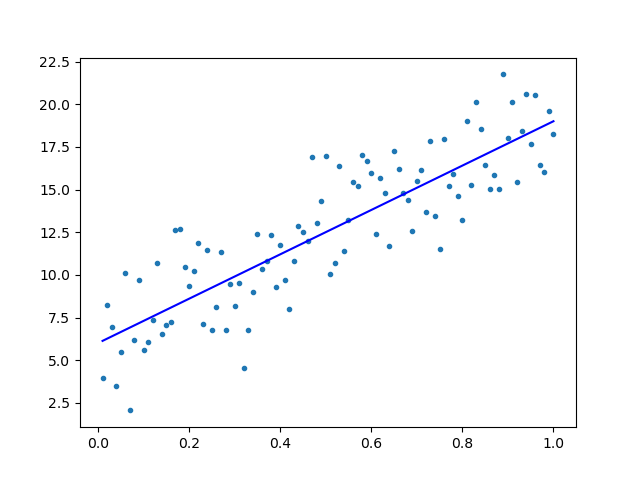
\includegraphics[width=0.7\linewidth]{linreg}
            \caption{Let us assume some measurements $(x_i,y_i),\ldots,(x_n,y_n)$ that lie approximately on a straight line.}
        \end{figure}
\end{frame}

\begin{frame}{Simple linear regression}
    In the simple linear regression, we assume that $\{x_i\}$ are fixed and that $Y_i$ are random variables:
    \[
        Y_i = \beta_0 + \beta_1 x_i + \varepsilon_i, \qquad i=1, \ldots, n 
    \]
    for some unknown parameters $\beta_0,\beta_1$ and $\{\varepsilon_i\}$ assumed independent with expectation value 0 and variance $\sigma^2$. We call $y=\beta_0+\beta_1x$ the {\em regression line}.
\end{frame}

\begin{frame}{Multiple Linear Regression}
    Here we have a response $Y$ that depends on a $d$-dimensional explanatory vector $\uvec{x}=[x_1,\ldots,x_d]^T$ via the relationship (for a single pair $(x,Y)$):
    \[
        Y = \beta_0 + \beta_1 x_1 + \cdots + \beta_d x_d +\varepsilon 
    \]
    And now the data lies approximately on a $d$-dimensional affine hyperplane
    \[y=\underbrace{\beta_0 + \beta_1 x_1 + \cdots + \beta_d x_d}_{g(\uvec{x}|\beta)}\]
    The function $g(\uvec{x}|\beta)$ is linear with respect to $\beta$ but not with respect to $\uvec{x}$. In order to facilitate the calculations (and coding) we can augment the feature vector with the constant $1$. 
\end{frame}

\begin{frame}{Multiple Linear Regression}
    If instead that a single pair $(x,Y)$, we consider the whole training set $\mathcal{T}=\{(\uvec{X}_1,Y_1),\ldots,(\uvec{X}_n,Y_n)\}$, by settling $\uvec{Y}=[Y_1,\ldots,Y_n]^T$ we can express the multiple linear regression modelfor the training set as:
    \[
        \uvec{Y}=\uvec{X}\beta+\varepsilon  
    \]
    where $\uvec{\varepsilon}=[\varepsilon_1,\ldots,\varepsilon_n]^T$ is a vector of iid copies of $\varepsilon$ and $\uvec{X}$ is the model matrix given by:
    \[
        \uvec{X}=
        \begin{pmatrix}
            1 & x_{11} & x_{12} & \cdots & x_{1d}\\
            1 & x_{21} & x_{22} & \cdots & x_{2d}\\
            \vdots & \vdots & \vdots & \vdots & \vdots\\
            1 & x_{n1} & x_{n2} & \cdots & x_{nd}\\
            \end{pmatrix}=
            \begin{pmatrix}
            1 & \uvec{x}_1^T\\
            1 & \uvec{x}_2^T\\
            \vdots & \vdots\\
            1 & \uvec{x}_n^T\\
            \end{pmatrix}  
    \]
\end{frame}


\begin{frame}{Multiple linear regression}
    \begin{figure}
        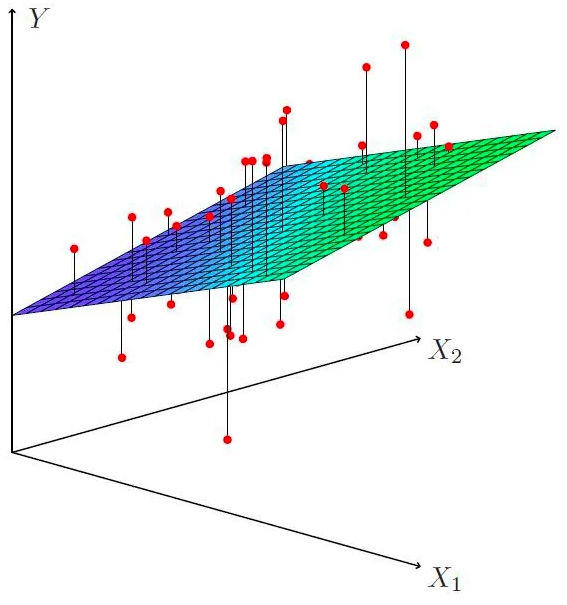
\includegraphics[width=0.6\linewidth]{hyperplane}
        \caption{\href{https://medium.com/analytics-vidhya/multiple-linear-regression-an-intuitive-approach-f874f7a6a7f9}{Example of multivariate linear regression}}
    \end{figure}
\end{frame}

\section{Analysis via linear models}

\begin{frame}{Parameter estimation}
    As we have seen, in the multiple linear regression model given by 
    \[
        \uvec{Y}=\uvec{X}\beta+\varepsilon   
    \]
$\uvec{X}$ is assumed to be fixed, and only $\uvec{Y}$ and $\varepsilon$ are random.

Thus, the model contains two different parameters: $\beta$ and $\sigma^2$ that need to be estimated from the training data $\tau$. Given a linear prediction function $g(\uvec{x})= \uvec{x}^T\uvec{\beta}$, the squarred error training loss is calculated as:
\[
    \mathscr{l}_{\tau}(g)=\frac{1}{n} \norm{\uvec{y}-\uvec{X}\beta}^2
\]
The optimal learner $g_{\tau}$ minimizes this expression, leading to the expression that yields $\uvec{\beta}$ through:
\[
    \uvec{X}^T \uvec{X} \beta = \uvec{X}^T \uvec{y}
\]
\end{frame}

\begin{frame}{Residuals}
    The traing loss can be then taken as an estimation of $\sigma^2$:
    \[
    \hat{\sigma^2}=\frac{1}{n} \norm{\uvec{y}-\uvec{X}\beta^2}
\]
The vector $\uvec{e}=\uvec{y}-\uvec{X}\uvec{\beta}$ is called the vector of residuals. $\norm{\uvec{e}}^2$ is called the residual sum of squares (RSS) and dividing RSS by $n-p$ gives an unbiassed estimate of $\sigma^2$, which we call the estimated residual squared error (RSE).
\end{frame}

\section{Feature selection}

\begin{frame}{Data over- and underfitting}
    \begin{figure}
        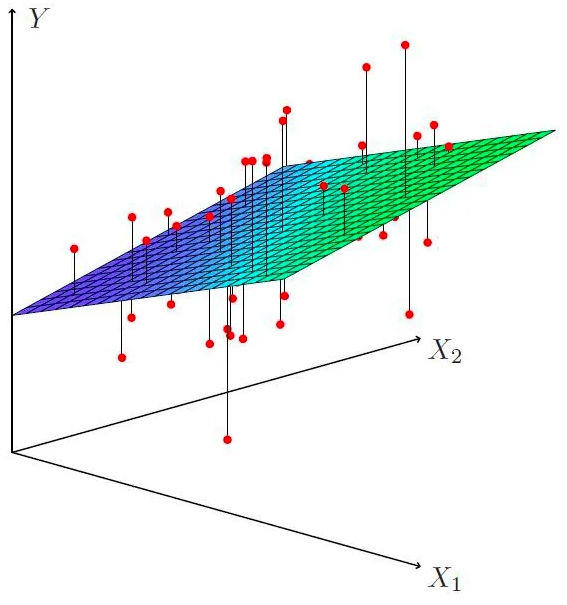
\includegraphics[width=0.4\linewidth]{hyperplane}
        \caption{Including too fw features leads to large approximation error (underfitting) and including too many to large statistical error (overfitting).This leads to the need for \href{https://www.simplilearn.com/tutorials/machine-learning-tutorial/feature-selection-in-machine-learning}{feauture selection}. Figure from \href{https://www.mathworks.com/discovery/overfitting.html}{Mathworks web site}.}
    \end{figure}

\end{frame}

\section{Bibliography}
\bibliographystyle{unsrt}
\bibliography{DataSciencewithPython}
\end{document}